First we will draw the graph for $n=1$ and $n=2$:\\
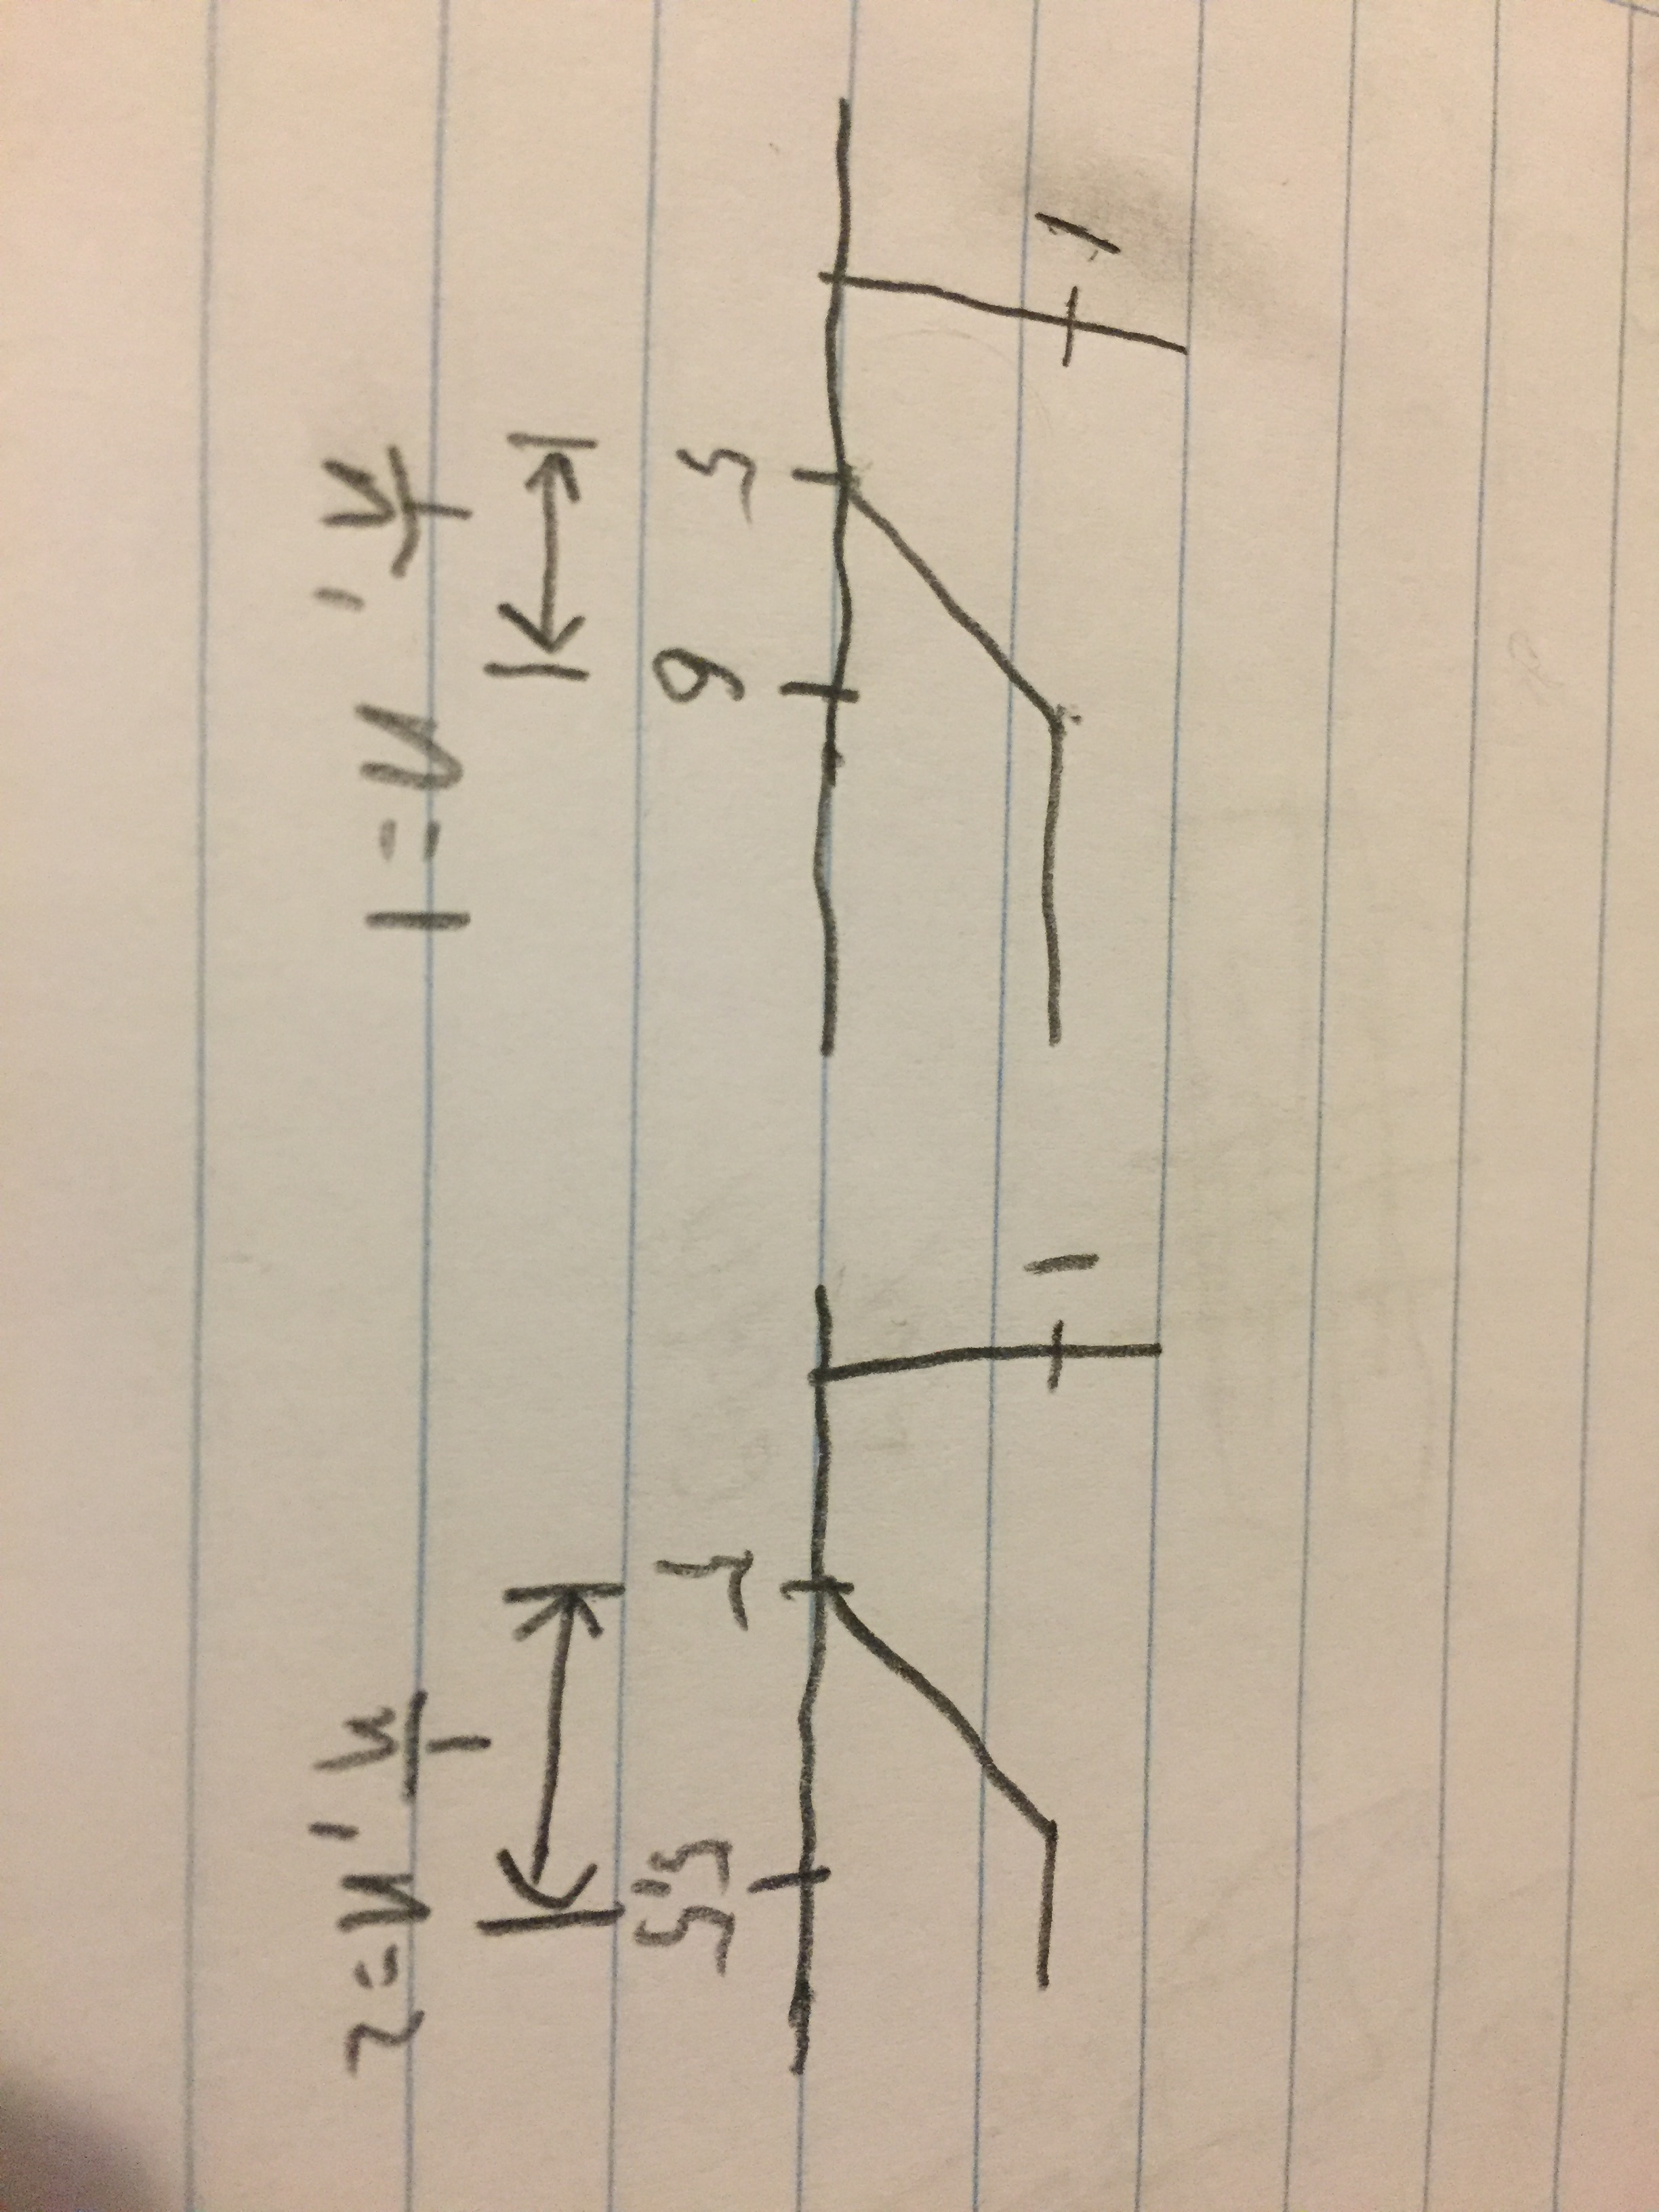
\includegraphics[angle=90,width=0.75\linewidth]{3b.jpg}\\
Then, we will write down our assumptions regarding the exercise text since it is not very precise:\\
We have to show that the following is true:
$$
F_n(X) \xrightarrow{\mathcal{L}} F(X) = 1, \textit{ for } X = 5
$$
We can prove that simply by looking at the graphs, and noticing what happens. We can see that the distance between the two points on the x-axis, $5$ and $5+\frac{1}{n}$ approaches zero as $n$ approaches infinity. This means that the value at $x=5$ also approaches 1:\\
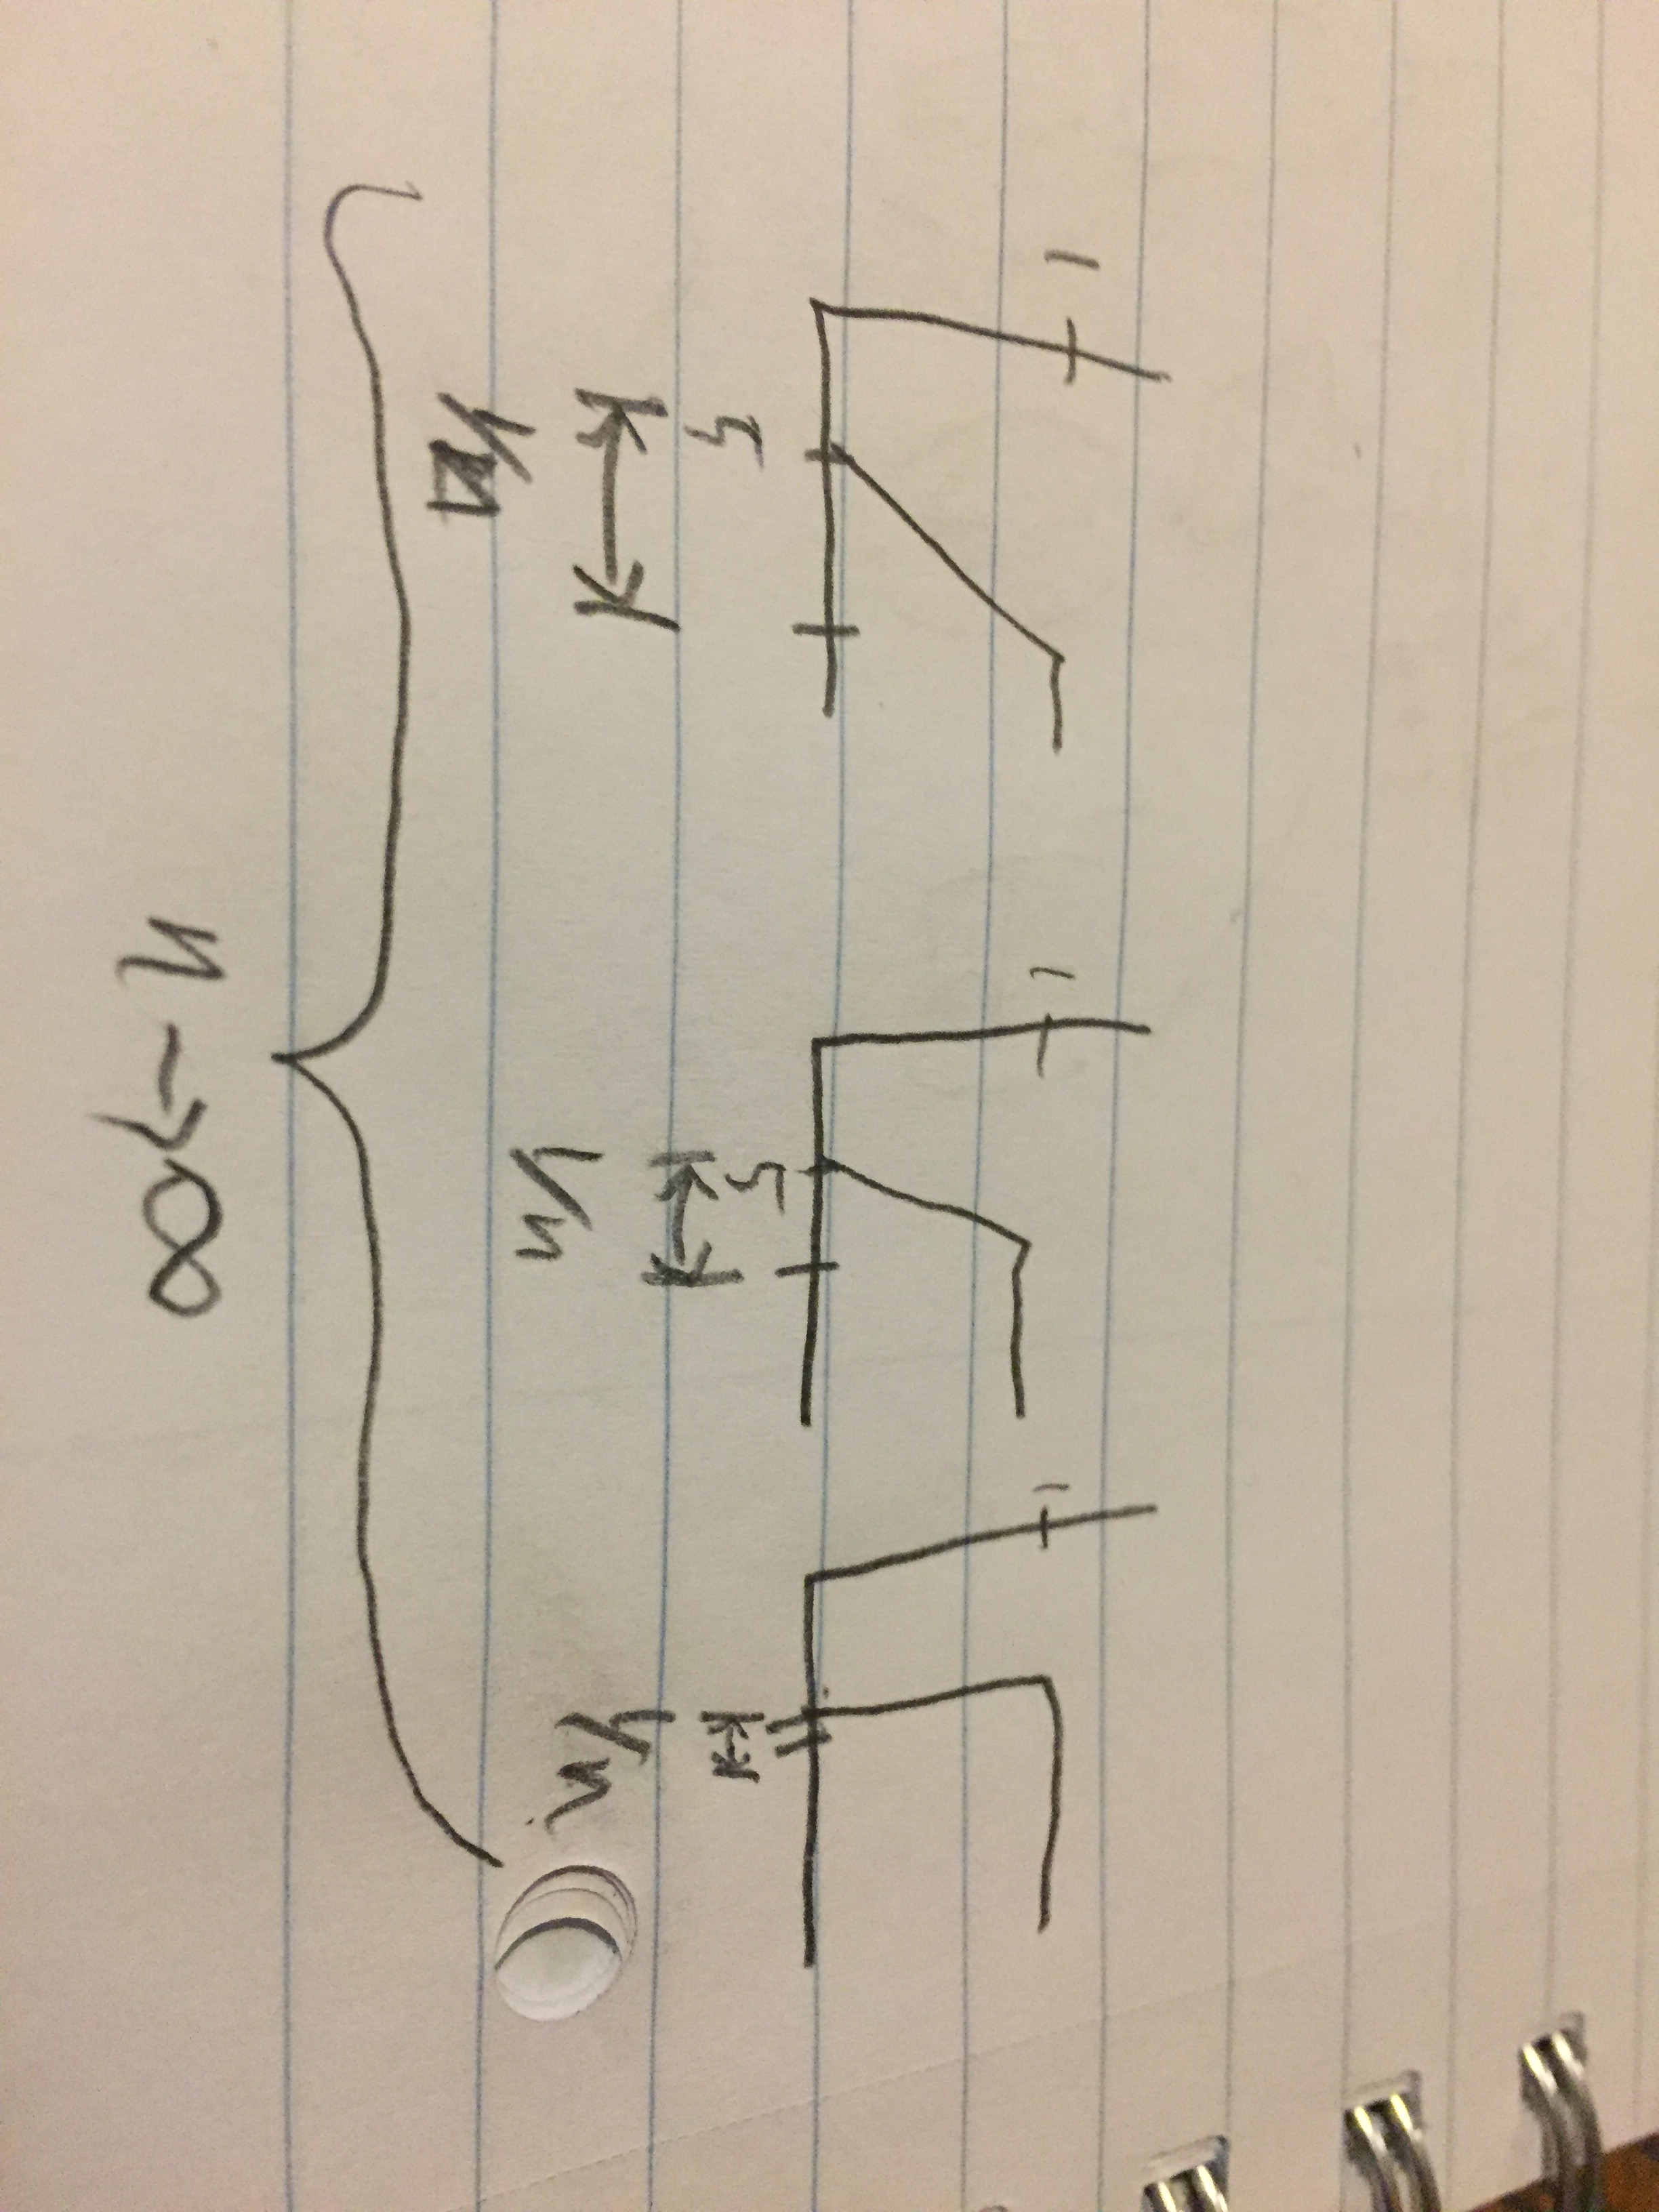
\includegraphics[angle=90,width=0.75\linewidth]{3b2.jpg}\\